\section{Spectral Theory} 

\subsection{Spectral Theory of General Mappings}

  \begin{definition}[Eigenvalue, Eigenvector]
    Let $A: V \longrightarrow V$ be a linear transformation over $\mathbb{F}$. If there exists a vector $v \in V$ such that
    \[ A v = \lambda v, \; \lambda \in \mathbb{F}\]
    then $a$ is called an \textbf{eigenvalue} of $A$, and $v$ is an \textbf{eigenvector} of $A$. Clearly, if a basis is realized for $V$ and $A$ is represented as a matrix, $v$ would have a basis representation. However, the value of $\lambda$ is invariant. The set of all eigenvalues 
    \[\lambda(A) \equiv \{ \lambda_1, \lambda_2, \cdots, \lambda_k\}\]
    is called the \textbf{spectrum} of $A$. 
  \end{definition}

  For a given eigenvalue $\lambda$ and its corresponding eigenvector $v$, it is clear that by linearity, every vector in $\Span v$ is an eigenvector, too. 

  Now that we have defined eigenvalues and eigenvectors, we first provide a visual description of these terms. Given a linear transformation $A: V \longrightarrow V$, we can visualize a certain basis of $V$ such that all the linear transformation $A$ does on that basis is merely extend or contract the basis vectors.

  \begin{definition}
    Given a $n \times n$ matrix $A$, the \textbf{characteristic polynomial} of $A$, denoted $p_A (t)$, is defined
    \[ p_A (t) \equiv \det{(A - t I)}\]
    The mapping $A \mapsto p_A (t)$ can be thought of as a mapping from Mat$(n, \mathbb{F}) \longrightarrow \mathbb{F}[t]$, where Mat$(n, \mathbb{F})$ is the algebra of $n \times n$ matrices over field $\mathbb{F}$, and $\mathbb{F}[t]$ is the polynomial algebra over $\mathbb{F}$. $p_A (t)$ is invariant under matrix similarity. 
  \end{definition}

  The motivation for defining such a polynomial is that it allows us to compute the eigenvalues of $A$. 

  \begin{definition}
    The \textbf{characteristic equation} of $A$ is defined by equating $p_A (t) = 0$. 
  \end{definition}

  \begin{theorem}
    The solutions of the characteristic equation of $A$ (i.e. the roots of $p_A (t)$) is precisely the spectrum of $A$. 
  \end{theorem}
  \begin{proof} 
    Bidirectional. 
    \begin{enumerate}
      \item $(\rightarrow)$ Let there be a $t = \lambda$ such that $p_A (\lambda) = 0 \iff \det{(A - \lambda I)} = 0$ which is equivalent to saying that ker$(A - \lambda I)$ is nontrivial. There must exist a $v \in $ ker$(A - \lambda I)$, meaning that $(A - \lambda I) v = 0 \iff A v = \lambda v$. By definition, $\lambda$ is an eigenvalue of $A$. 
      \item $(\leftarrow)$ This reasoning can be extended in the opposite direction. 
    \end{enumerate}
  \end{proof}

  \begin{theorem}
    Eigenvectors of a linear transformation $A$ corresponding to different eigenvalues are linearly independent, but not necessarily orthogonal. It follows that if the characteristic polynomial of a $n \times n$ matrix $A$ has $n$ distinct roots, then $A$ has $n$ linearly independent eigenvectors. 
  \end{theorem}
  \begin{proof}
    Simple, by contradiction.
  \end{proof}

  \begin{example}
    It is clear that the Fibonacci sequence can be produced with matrix multiplication as such 
    \[ \begin{pmatrix}
    a_{n+1} \\ a_n
    \end{pmatrix} = A^n \begin{pmatrix}
    a_1 \\ a_0
    \end{pmatrix} = \begin{pmatrix}
    1&1\\1&0
    \end{pmatrix}^n \begin{pmatrix}
    1\\1
    \end{pmatrix}\]
    Given that 
    \[\lambda_1 = \frac{1+\sqrt{5}}{2}, \; \lambda_2 = \frac{1 - \sqrt{5}}{2}\]
    we can diagonalize $A$ into the form 
    \[A = \begin{pmatrix}
    \frac{1}{\lambda_1 - \lambda_2} & \frac{\lambda_2}{\lambda_2 - \lambda_1} \\
    \frac{1}{\lambda_2 - \lambda_1} & \frac{\lambda_1}{\lambda_1 - \lambda_2}
    \end{pmatrix} \begin{pmatrix}
    \lambda_1 & 0 \\ 0 & \lambda_2 
    \end{pmatrix} \begin{pmatrix}
    \lambda_1 & \lambda_2 \\
    1 & 1
    \end{pmatrix} \implies A^n = S^{-1} \begin{pmatrix}
    \lambda_1^n & 0 \\ 0 & \lambda_2^n 
    \end{pmatrix} S\]
    which implies that after evaluating, we get 
    \[ a_n = \frac{1}{\sqrt{5}} \bigg( \Big(\frac{1+\sqrt{5}}{2}\Big)^n - \Big(\frac{1-\sqrt{5}}{2}\Big)^n \bigg)\]
    This is a surprising result since it also says that the expression above is always an integer for all natural number $n$. 
  \end{example}

  \begin{definition}
    Given a subspace $U_1 \subset U$ and linear transformation $T: U \longrightarrow U$. We say that $U_1$ is \textbf{invariant} under $T$ if 
    \[u \in U_1 \implies T u \in U_1\]
  \end{definition}

  \begin{theorem} 
    Let $a_1, a_2, \cdots, a_n$ be the eigenvalues of $A$. Then 
    \[\sum_i a_i = \Tr{A}, \;\;\; \prod_i a_i = \det{A}\]
  \end{theorem}
  \begin{proof}
    The mapping $A \mapsto \det{(A - x I)}$ is a mapping from the set of $n \times n$ matrices to the polynomial algebra $\mathbb{F}[x]$. Direct application of the Viete's formulas in $\mathbb{F}[x]$ produces the statement and this result can be extended to the rest of the formulas. 
  \end{proof}

  \begin{theorem}[Spectral Mapping Theorem]
    Let $q$ be any polynomial, $A$ a square matrix with an eigenvalue $a$. Then: 
    \begin{enumerate}
      \item $q(a)$ is an eigenvalue of $q(A)$. 
      \item Every eigenvalue $q(A)$ is of the form $q(a)$, where $a$ is an eigenvalue of $A$. 
    \end{enumerate}
  \end{theorem}
  \begin{proof} 
    Listed. 
    \begin{enumerate}
      \item Let $h$ be an eigenvector of A with corresponding eigenvalue $a$. 
      \begin{align*}
          Ah = ah & \implies A^{2} h = Aah = aAh = a^{2} h \\
           & \implies A^{n} h = a^{n} h   \\
           & \implies q(A)h = q(a)h \\
           & \implies q(a) \text{ is an eigenvalue of }q(A)
      \end{align*}
      \item Let $p$ be the eigenvalue of $q(A) \iff \det{\big(q(A) - p I\big)} = 0$. We expand: 
        \begin{equation}
          q(s) - p = c\prod \big(s-r_{i}\big), r_{i} \in \mathbb{C}
        \end{equation}
        Replacing the variable $s$ with $A$, we have
        \begin{equation}
          q(A) - pI = c \prod \big(A-r_{i}I\big)
        \end{equation}
        Since $\det{\big( q(A) - pI\big)} = 0$, at least one $r_{i}$, say $r_{k}$ exists such that $\det{\big( A - r_{k} I \big)} = 0 \iff r_{k}$ is an eigenvalue of $A$. Since $q(r_{j})-p = 0$, $p = q(r_{j})$ is an eigenvalue of $q(A)$. 
    \end{enumerate}
  \end{proof}

  The following theorem is an equivalent version of the spectral mapping theorem.

  \begin{theorem}
    Let $A$ be a $n \times n$ matrix and let $f$ be a polynomial. If the chracteristic polynomial of $A$ has factorization 
    \[p_A (t) = \prod_{i = 1}^n (t - \lambda_i)\]
    then the characteristic polynomial of the matrix $f(A)$ is given by 
    \[p_{f(a)} (t) = \prod_{i = 1}^n (t - f(\lambda_i))\]
  \end{theorem}

  We can actually create a bound on the spectrum of a square matrix. 

  \begin{theorem}[Gershgorin Circle Theorem]
    Let $A \in $ Mat$(n, \mathbb{C})$ with entries $a_{i j}$. Let $R_i = \sum_{i \neq j} |a_{i j}|$ be the sum of the absolute values of the non-diagonal entries of the $i$th row, and let $D_(a_{i i}, R_i) \subset \mathbb{C}$ be a closed disk with radius $R_i$ centered at $a_{i i}$ in the complex plane, called a \textbf{Gershgorin Disk}. Then every eigenvalue of $A$ lies within the union of all $n$ Gershgorin Disks. That is, 
    \[ \lambda_j (A) \in \bigcup_{i= 1}^{n} D_(a_{i i}, R_i) \subset \mathbb{C}, \text{ for all } j\]
  \end{theorem}
  \begin{proof}
    Let $\lambda$ be an eigenvalue of $A$ with its eigenvector $v = (v_j)$. Scale $v$ by multiplying it by $ \pm 1 / \max{\{|v_j|\}_j}$ to get a vector $x$ with its maximal entry $x_i = 1$ and $|x_j| \leq 1, \; j \neq i$. Then, 
    \[A x = \lambda x \implies \sum_{j} a_{i j} x_j = \lambda x_i = \lambda \implies \sum_{j \neq i} a_{i j} x_j + a_{i i} = \lambda\]
    Applying the triangle inequality, 
    \[| \lambda - a_{i i} | = \bigg| \sum_{j \neq i} a_{i j} x_j\bigg| \leq \sum_{j \neq i} |a_{i j}| |x_j| \leq \sum_{j \neq i} |a_{i j}| = R_i\]
  \end{proof}

  \begin{corollary}
    The eigenvalues of $A$ must also lie within the Gershgorin discs $C_j$ corresponding to the columns of $A$. 
  \end{corollary}
  \begin{proof}
    This is a direct result from the fact that $A$ is similar to $A^T$. Alternatively, we can apply the same process in the proof above to $A^T$.
  \end{proof} 

  If one observes that the off-diagonal entries of $A$ are small in absolute value, it can be concluded that the diagonal entries are "close" to the true eigenvalues of $A$. $A$ is diagonal if and only if the Gershgorin disks are points. 

  \begin{theorem}[Cayley Hamilton]
    Every matrix $A$ satisfies its own characteristic equation. That is, 
    \[ p_{A}(A) = 0\]
  \end{theorem} 

\subsection{Eigendecompositions and Jordan Normal Form}

  However, the entire concept of matrices are not fully grasped with just eigenvectors. If it were, then linear algebra would be a much simpler matter. To extend our toolkit, we must introduce generalized eigenvectors. From here, we will assume that our field is over $\mathbb{C}$. We use the fact that the field is over $\mathbb{C}$ because it allows us to claim that the characteristic polynomial in $\mathbb{C}[t]$ can be factored into linear components, by the fundamental theorem of algebra. 

  \begin{definition}
    A genuine eigenvector of $A$ satisfies $(A-aI)h = 0$. A \textbf{generalized eigenvector} $f$ satisfies $(A-a I)^{d} f = 0$ for some $d \geq 1$. 
  \end{definition}

  To provide a visual intuition of how generalized eigenvectors transform under $A$, observe that 
  \begin{align}
    (A - aI) h = 0 \text{ and } (A - aI)^2 f = 0 & \implies (A - aI)^f = h \\
    & \implies A f = a f + h, \; Ah = ah \\
    & \implies A^2 f = a A f + A h = a^2 f + 2 a h \\
    & \implies A^N f = A^N f + N a^{N-1} h 
  \end{align}

  This implies that the generalized eigenvector is first scaled by a factor of $a$, similar to a genuine eigenvector, but then a factor of the genuine eigenvector is then added to the scaled generalized one. Note that in higher dimensions of $N$, a greater multiple of $h$ must be added after scaling $f$. 

  This means that given an eigenvalue $\lambda$, there is always at least one genuine eigenvalue associated with $\lambda$. Furthermore, there may be additional generalized eigenvectors also corresponding to $\lambda$. This leads to the following definition

  \begin{definition}
    The subspace formed by the span of the generalized (and genuine) eigenvectors of $\lambda$ form what is called the \textbf{eigenspace associated with $\lambda$}, denoted $E(\lambda)$. 
  \end{definition}

  We can measure the characteristics of the eigenspaces with the following definitions. 

  \begin{definition}
    The \textbf{algebraic multiplicity} of an eigenvalue $\lambda$ is the dimension of its eigenspace. It is precisely
    \[\dim{E(\lambda)}\]  
    In order to compute the algebraic multiplicity of $\lambda_i$ in $A$, we find the maximal value of $d_i$ such that $(t-\lambda)^{d_i}$ divides $p_A (t)$. With this, we can define 
    \[E(\lambda) = \ker{(A - \lambda_i I)^{d_i}}\]
  \end{definition} 

  \begin{theorem}
    Given $A: V \longrightarrow V$ with eigenspaces $E(\lambda_1), E(\lambda_2), \cdots, E(\lambda_k)$, 
    \[E(\lambda_1) \oplus E(\lambda_2) \oplus \cdots \oplus E(\lambda_k) = V\]
    That is, every vector $v \in V$ can be uniquely expressed as the sum 
    \[ v = h_1 + h_2 + \cdots + h_k, \; h_i \in E(\lambda_i)\]
    this is called the \textbf{eigenbasis of $V$}. 
  \end{theorem}
  \begin{proof}
    The definition of algebraic multiplicity implies that each eigenspace is disjoint except at $0$ and that their dimensions sum to $\dim{V}$. 
  \end{proof}

  \begin{definition}
    The \textbf{geometric multiplicity} of an eigenvalue $\lambda$ of a linear transformation $A$ is the dimension of the span of genuine eigenvectors in its eigenspace. It is precisely 
    \[\dim{\ker{(A - \lambda I)}}\]
    Note that since the span of genuine eigenvectors is a subspace of $E(\lambda)$, the geometric multiplicity is always less than or equal to the algebraic multiplicity. 
  \end{definition}

  Now we are ready to introduce the eigendecomposition of a linear mapping $A$.

  \begin{theorem}
    Given a linear mapping $A$ with its eigenvalues $\lambda_1, \ldots, \lambda_k$ and associated eigenspaces $E(\lambda_1), \ldots, E(\lambda_k)$, $A$ maps each eigenspace to itself. That is, 
    \[A\big( E(\lambda_i) \big) \subset E(\lambda_i), \; i = 1, 2, \cdots, k\]
  \end{theorem}

  \begin{corollary}[Jordan Normal Form]
    Every linear mapping $A: V \longrightarrow V$ can be decomposed into the sum of the linear mappings of each eigenspace $E(\lambda_i)$. That is, it can be expressed in the form 
    \[A: \prod_i E(\lambda_i) \longrightarrow \prod_i E(\lambda_i)\]
    which we can define, given $h_i \in E(\lambda_i)$, 
    \[A(v) = A\bigg(\sum_i h_i \bigg) = \sum_i A(h_i), \; A(h_i) \in E(\lambda_i) \]
  \end{corollary}

  The process of eigendecomposition for a linear mapping $A$ is really just a clever change of basis for the $n \times n$ matrix representation of $A$ over $\mathbb{C}$, where the new basis is now the set of genuine and generalized eigenvectors. The new matrix formed by performing the change of basis on matrix $A$ is called the \textbf{Jordan Normal Form}, or \textbf{Jordan Canonical Form}, of $A$. We will now describe the construction of the JNF of an arbitrary $n \times n$ matrix. 

  It is actually simple. Let the eigenvalues of the matrix $A$ be $\lambda_1, \lambda_2, \cdots, \lambda_k$, with its associated eigenspaces $E(\lambda_i)$. Let the algebraic multiplicity of eigenspace $E(\lambda_i)$ be $alg_i$. Then, every $n \times n$ matrix over $\mathbb{C}$ has the block form 
  \begin{equation}
    J = \begin{pmatrix}
      A_1&0&0&0\\
      0&A_2&0&0\\
      0&0&\cdots&0\\
      0&0&0&A_k
    \end{pmatrix}
  \end{equation}

  where each block $A_i$ represents the transformation in $E(\lambda_i)$. This means that each $A_i$ must be an $alg_i \times alg_i$ submatrix. The definition of the generalized eigenvectors shown in equation $(11)$ shows that each block must be of form 
  \begin{equation}
    A_i = \begin{pmatrix}
      \lambda_i & 1 & 0 & \cdots & 0\\
      0 &\lambda_i & 1 &\cdots&0 \\
      0&0&\lambda_i&\cdots&0\\
      \cdots&\cdots&\cdots&\cdots&1\\
      0&0&\cdots&0&\lambda_i
    \end{pmatrix}
  \end{equation}

  With $\lambda_i$'s in the main diagonal and $1$'s in the superdiagonal of $A_i$. The first column of $A$ refers to the transformation of the genuine eigenvector, while the other columns refers to the transformation of the generalized eigenvectors, where $\lambda_i$ refers to the scaling of the $d$th generalized eigenvector and the $1$ refers to the adding of the $(d-1)$th generalized eigenvector to the scaled $d$th vector. If there are no generalized eigenvectors in an eigenspace $E(\lambda_i)$, then $A_i$ is a $1 \times 1$ matrix $( \lambda_i )$. Observe that this form is consistent with our previous theorems, especially the fact that $A$ maps distinct eigenspaces to themselves. 

  Finally, the change of basis is represented through the matrix multiplication. 
  \[J = P^{-1} A P, \; P = \begin{pmatrix}
  |&|&|&| \\ 
  f_1&f_2&\cdots&f_n \\
  |&|&|&|
  \end{pmatrix} \]
  where $f_i$ is the genuine/generalized eigenvectors corresponding to the transformation represented in the $i$th column of $J$. The Jordan Normal Form of a matrix is unique up to the permutations of its diagonal blocks. 

  Notice that the Jordan Normal Form must be an $n \times n$ matrices over $\mathbb{C}$, not $\mathbb{R}$. However, given a matrix $A$ over $\mathbb{R}$, we can construct a similar block diagonal form over $\mathbb{R}$. Since $A$ is real $\implies p_A (t) \in \mathbb{R}[t]$, $\mu \in \mathbb{C}$ is a root of $p_A$ implies that $\bar{\mu}$ is also a root. This means that in the case where $\mu = a \pm b i$ is a pair of complex eigenvectors with eigenvectors $z$ and $\bar{z}$. The associated $2 \times 2$ Jordan block will be of form
  \[\begin{pmatrix}
  a&-b\\ b&a
  \end{pmatrix}\]

  with the associated column vectors in $P$ being
  \[v_1 = \frac{z + \bar{z}}{2}, \; v_2 = \frac{i (z - \bar{z})}{2}\]

  Notice that $z \in \mathbb{C}^n$ is a complex eigenvector belonging to complex eigenvalue $\mu$, and we make the best "approximations" of $z, \bar{z}$ and $\mu, \bar{\mu}$ with the new real vectors $v_1$ and $v_2$. Note that the Jordan block states that
  \[A(v_1) = a v_1 + b v_2, \; A(v_2) = -b v_1 + a v_2\]
  which is true since 
  \begin{align*}
      A(v_1) = A\Big( \frac{z + \bar{z}}{2} \Big) & = \frac{1}{2} \big( A(z) + A(\bar{z}) \big) \\
      & = \frac{1}{2}\big( (a+bi)z + (a-bi) \bar{z} \big) \\
      & = \frac{1}{2} \big( (a)(z + \bar{z}) + (bi) (z - \bar{z})\big) \\
      & = a \frac{z + \bar{z}}{2} + b \frac{i(z-\bar{z}}{2} = a v_1 + b v_2 \\
  \end{align*}
  and 
  \begin{align*}
      A(v_2) = A \Big( \frac{i(z-\bar{z})}{2} \Big) & = \frac{i}{2} \big( A(z) - A(\bar{z}) \big) \\
      & = \frac{i}{2} \big( (a+bi) z - (a-bi) \bar{z}\big) \\
      & = \frac{i}{2} \big( (a) (z - \bar{z}) + (bi)(z+\bar{z})\big) \\
      & = a \frac{i(z-\bar{z})}{2} - b \frac{z + \bar{z}}{2} = a v_2 - b v_1
  \end{align*}
  It suffices to only modify this case for $2 \times 2$ blocks because all complex eigenvalues of real matrices must come in conjugate pairs (but this is not necessarily true for complex matrices, which have characteristic polynomials in $\mathbb{C}[t]$). 

  \begin{corollary}
    The following $2 \times 2$ Jordan block of the form shown below can be turned into the complex Jordan block and vice versa. 
    \[\begin{pmatrix}
    \cos{\theta} & -\sin{\theta} \\
    \sin{\theta} & \cos{\theta} 
    \end{pmatrix} \xleftrightarrow{} \begin{pmatrix}
    e^{i \theta} & 0 \\
    0 & e^{- i \theta}
    \end{pmatrix}\]
  \end{corollary}

  However, there could be bigger Jordan blocks of generalized eigenspaces corresponding to conjugate pairs. Observe the following JNF, with columns (from left to right) corresponding to the transformations $h_1$ (genuine), $k_1$ (generalized), $h_2$ (genuine), and $k_2$ generalized). 
  \[\begin{pmatrix}
  e^{i \theta} & 1 & & \\
  & e^{i \theta} & & \\
  & & e^{-i \theta} & 1 \\
  & & & e^{i- \theta}
  \end{pmatrix}\]
  Using the corollary shown above, we can modify the eigenvalues and eigenvectors into real values and construct the simplest "real form" (assuming $i \neq 0, \pi$) of the matrix 
  \[\begin{pmatrix}
  \cos{\theta} & - \sin{\theta} & 1 & 0 \\
  \sin{\theta} & \cos{\theta} & 0 & 1 \\
  0 & 0 & \cos{\theta} & - \sin{\theta} \\
  0 & 0 & \sin{\theta} & \cos{\theta}
  \end{pmatrix}\]
  where the columns (from left left to right) now correspond to transformation of real eigenvectors
  \[\frac{h_1 + h_2}{2}, \frac{i(h_1 - h_2)}{2}, \frac{k_1 + k_2}{2}, \frac{i(k_1 - k_2)}{2}\]
  Therefore, we can state that the linear transformation represented by the two matrices in their respective bases are equivalent. 

  \begin{example}[Rotation Around Vector]
    \begin{figure}[H]
      \centering 
      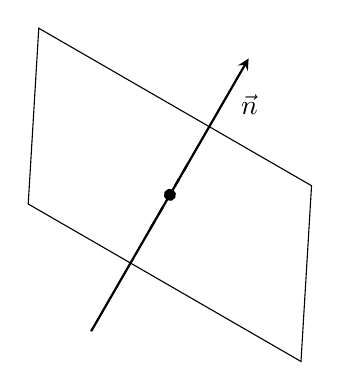
\begin{tikzpicture}
        % Rotate the entire picture 30 degrees clockwise
        \begin{scope}[rotate=-30]
          % Define coordinates for the parallelogram
          \coordinate (A) at (-2,-1);
          \coordinate (B) at (2,-1);
          \coordinate (C) at (1,1);
          \coordinate (D) at (-3,1);
          
          % Draw the parallelogram
          \draw (A) -- (B) -- (C) -- (D) -- cycle;
          
          % Draw the normal vector line
          \draw[-stealth, thick] (-0.5,-2) -- (-0.5,2);
          
          % Draw the dashed portion where the line intersects the parallelogram
          \draw[dashed, thick] (-0.5,-0.5) -- (-0.5,0.5);
          
          % Add a dot at intersection point
          \filldraw (-0.5,0) circle (2pt);
          
          % Label the normal vector
          \node at (-0.2,1.5) {$\vec{n}$};
        \end{scope}
      \end{tikzpicture}
      \caption{The linear operator that rotates around a vector $v$ by an angle $\theta$ has an eigendecomposition of the span of $v$ as shown (with eigenvalue $1$) and the 2-dimensional plane (having two complex eigenvalues). } 
      \label{fig:rotation}
    \end{figure}
  \end{example}

  \begin{definition}
    A matrix is \textbf{diagonalizable} if we can perform a change of basis on it to create a diagonal matrix. 
  \end{definition}

  \begin{theorem}
    A matrix is diagonalizable if and only if its algebraic multiplicities is equal to its geometric multiplicities. That is, if the matrix only has genuine eigenvectors. This is also equivalent to saying that all of $A$'s eigenspaces have dimension $1$. 
  \end{theorem}

  It is clear that since eigendecompositions are intrinsic to linear mappings, the JNF of similar matrices are the same. That is, the eigenvalues and the dimensions of the eigenspaces are invariant under a change of basis. 

  \begin{theorem}
    Two matrices are similar if and only if their eigendecompositions are the same. That is, if they have the same eigenvalues and the dimensions of the corresponding eigenspaces are the same. 
  \end{theorem}
  \begin{proof}
    $(\rightarrow)$ $A \sim B \implies A = S^{-1} B S = S^{-1} P^{-1} J P S = (PS)^{-1} J (PS) \implies$ JNF of $A$ and $B$ are the same.  \\
    $(\leftarrow)$ $A$ and $B$ have same JNF $\implies A = P^{-1} J P, B = Q^{-1} J Q \implies J = Q B Q^{-1} \implies A = P^{-1} Q B Q^{-1} P = (Q^{-1} P)^{-1} B (Q^{-1} P) \implies A \sim B$. 
  \end{proof}

  \begin{theorem}
    $A \sim A^T$. 
  \end{theorem}
  \begin{proof}
    By the theorem above, it is sufficient to prove that $A$ and $A^T$ have the same eigendecomposition. Since $(A - \lambda I)^T = A^T - \lambda I$, $\det{(A - \lambda I)} = 0 \iff \det{(A - \lambda I)^T} = \det{(A^T - \lambda I)} \implies $ $A$ and $A^T$ have the same eigenvalues. Similarly, $\big( (A - \lambda I)^d \big)^T = (A^T - \lambda I)^d \implies$ the eigenspaces of $A$ and $A^T$ have the same dimension. 
  \end{proof}

\subsection{Spectral Theory of Self-Adjoint Maps}

\subsection{Positive Definite Maps}

  \begin{definition}[Spectral Radius]
    The \textbf{spectral radius} of $A$ is defined
    \begin{equation}
      r(A) \equiv \max_i |a_i|, \; a_i \text{ are eigenvalues}
    \end{equation}
  \end{definition}

  \begin{definition}[Positive-Semidefinite]
    A self-adjoint linear mapping $H$ from a real or complex Euclidean space onto itself is \textbf{positive definite} if 
    \begin{equation}
      (x, H x) > 0 \text{ for all } x \neq 0
    \end{equation}
    $H$ is called \textbf{positive semidefinite} if 
    \begin{equation}
      (x, H x) \geq 0
    \end{equation}
  \end{definition}

  \begin{theorem}[Properties of Positive Definite Matrices] 
    Here we state basic properties. 
    \begin{enumerate}
      \item $I$ is positive definite. 
      \item Positive mappings form a subspace in the space of linear mappings. 
      \begin{align*}
        &M, N \text{ positive} \implies M + N \text{ is positive} \\
        &M \text{ positive} \implies a M \text{ is positive for all} a \in \mathbb{F}
      \end{align*}
      \item $H$ positive and $Q$ invertible $\implies Q^\dagger H Q$ positive. 
    \end{enumerate}
  \end{theorem}

  \begin{theorem}
    $H$ is positive definite if and only if all of its eigenvalues are positive. Furthermore, every positive mapping is invertible.
  \end{theorem}

  \begin{theorem}
    Every positive mapping $M$ has a unique positive square root. That is, there exists a unique positive mapping $N$ such that
    \begin{equation}
      N^2 = M 
    \end{equation}
    We denote $N$ as $\sqrt{M}$. 
  \end{theorem}

  \begin{definition}
    Given that $M, N$ are positive definite mappings. 
    \begin{equation}
      M > N \iff M - N > 0, \text{ that is, $M$ is positive}
    \end{equation}
  \end{definition}

  \begin{theorem}
    If $M, N$ are positive definite mappings 
    \begin{equation}
       M > N \implies M^{-1} < N^{-1}
    \end{equation}
  \end{theorem}

  \begin{theorem}
    In $\mathbb{R}^n$ endowed with the dot product, a $n \times n$ matrix $A$ is positive definite if and only if 
    \begin{equation}
      (x, A y) = x^T A y > 0 
    \end{equation}
    for every $x, y \in \mathbb{R}^n$. $A$ is positive semi-definite if and only if 
    \begin{equation}
      (x, A y) = x^T A y \geq 0
    \end{equation}
  \end{theorem}

  The following is a useful fact regarding inner products of $\mathbb{R}^n$. 

  \begin{theorem}
    The set of all inner products that can be defined on $\mathbb{R}^n$ is bijective to the set of positive-definite symmetric $n \times n$ matrices $A$ (which is itself bijective to the set of all positive-definite mappings). That is, every inner product of $\mathbb{R}^n$ can be defined 
    \begin{equation}
      (x, y) \equiv x^T A y
    \end{equation}
    Note that when $A = I_n$, the inner product is the regular dot product.
  \end{theorem}

\subsection{Singular Value Decomposition} 

  We now proceed to another crucial decomposition, called the singular value decomposition. While the JNF allows us to choose the most convenient choice of basis for a square matrix, the Singular Value Decomposition (SVD) allows us to decompose general $m \times n$ matrices. 

  \begin{theorem}[Singular Value Decomposition]
    Any linear mapping $M$ from an $n$-dimensional inner product space to a $m$-dimensional inner product space can be decomposed into 
    \begin{equation}
      M = U \Sigma V^\dagger = \begin{pmatrix}
       \vert & \vert & \vert & \vert\\
      y_1 & y_2 & \ldots & y_m \\
      \vert & \vert & \vert & \vert
      \end{pmatrix}\begin{pmatrix}
      \sigma_1 & & & &0\\
      &\ddots &&& \vdots \\
      & & \sigma_p & & 0\\
      & & & \ddots &\vdots \\
      0 & \ldots &0& \ldots &0
      \end{pmatrix} \begin{pmatrix}
      \text{---}&x_1&\text{---} \\
      \text{---}&x_2&\text{---} \\
      \text{---}&\vdots&\text{---} \\
      \text{---}&x_n&\text{---}
      \end{pmatrix}
    \end{equation}
    where $U \in U(m), V \in U(n)$ and $\Sigma$ has diagonal elements with nonnegative real entries. Also, $p = $ rank$(M) \leq \min{\{n,m\}}$. This form is known as the \textbf{singular value decomposition}. The columns of $U$, denoted $y_i$, are called the \textbf{left singular vectors} and the columns of $V$ (i.e. the rows of $V^\dagger$), denoted $x_i$, are called the \textbf{right singular vectors}. The diagonal entries of $\Sigma$ are called the \textbf{singular values}. The SVD is unique up to the order of singular values, but it is generally constructed so that $\sigma_1 \geq \sigma_2 \geq \ldots \geq \sigma_p$. 
  \end{theorem}

  To provide a brief, yet unrigorous, justificiation of why the SVD exists, we look at the linear mapping $M: X \longrightarrow Y$, with $\dim{X} = n, \dim{Y} = m$. If $M$ is injective $(\iff m \geq n)$, given the basis $\{e_i\}$ for $X$, we can complete the linearly independent set $\{Me_i\}_{i=1}^n$ to a basis in $Y$ and represent $M$ as the mapping
  \begin{equation}
    \Sigma_{inj} = \begin{pmatrix} &&\\ &I_n&\\ &&\\ 0&\ldots &0 \end{pmatrix}
  \end{equation}
  If $M$ is surjective $(\iff m \leq n)$, then given basis $\{f_i\}_{i=1}^m$ of $Y$, we can choose a basis $\{e_j\}_{j=1}^n$ of $X$ such that $M(e_i) = f_i (i = 1, 2, \ldots, m)$, and $M(e_i) = 0$ when $i > m$. This produces the matrix
  \begin{equation}
    \Sigma_{surj} = \begin{pmatrix} &&&0\\&I_m&& \vdots \\&&&0\end{pmatrix}
  \end{equation}
  We now present the following theorem without proof. 

  \begin{theorem}
    Any map $M: X \longrightarrow Y$ can be written as a surjective map followed by an injective map. 
  \end{theorem}

  This theorem implies that any map, when given the right choice of basis, can be written as 
  \begin{equation}
    \Sigma_{inj} \Sigma_{surj} = \begin{pmatrix}
    &&&\cdots&0\\
    &I_p&&\cdots&0\\
    &&&\cdots&\cdots\\
    \cdots&\cdots&\cdots&\cdots&0\\
    0&0&\cdots&0&0
    \end{pmatrix} = \begin{pmatrix}
    1&&&&0\\
    &\cdots&&&\cdots\\
    &&1&&0\\
    &&&\cdots&\cdots\\
    0&\cdots&0&\cdots&0
    \end{pmatrix}
  \end{equation}
  where rk$(M) = p = $ the number of $1$'s in $\Sigma_{inj} \Sigma_{surj}$. As for choosing the proper set basis for $X$ and $Y$, we can find these passive transformations in the unitary groups $U(n)$ and $U(m)$. 

  We now present a geometric description of the singular value decomposition. Think of the unit $n$-ball being rotated and flipped ($V^\dagger$ applied) under the unitary transformation. Then, it is stretched along its othogonal axes to result in an ellipsoid living in an $m$-dimensional space. The factor of stretching and compressing the axes are precisely the singular values. Finally, this ellipsoid is rotated and flipped ($U$ applied) back to its original basis. 

  \begin{theorem}
    Geometrically, we can see that the largest singular value is the matrix norm, also called the operator norm. 
    \begin{equation}
      \|M\| = \sigma_1
    \end{equation}
  \end{theorem}

  \begin{theorem}[Properties of Singular Values] 
    Given linear mapping $A$ from a $n$-dimensional inner product space to $m$-dimensional inner product space, 
    \begin{enumerate}
      \item $\sigma_i(A) = \sigma_i (A^T) = \sigma_i (A^\dagger) = \sigma_i (\bar{A})$

      \item $\forall \; U \in U(m), V \in U(n), \; \sigma_i (A) = \sigma_i (U A V)$

      \item Relation to eigenvalues
      \begin{equation}
        \sigma_i^2(A) = \lambda_i (A^\dagger A) = \lambda_i (A A^\dagger)
      \end{equation}
    \end{enumerate}
  \end{theorem}

  We now present the (not the best) process of computing SVD of small matrices by hand. Given matrix $M$, $M = U \Sigma V^\dagger \implies M^\dagger M = V \Sigma^2 V^\dagger$. The eigenvalues of $M^\dagger M$ are $\sigma_i^2$ with corresponding eigenvectors being the columns of $V$, which can all be found by putting $M^\dagger M$ into JNF. We repeat this process for $M M^\dagger = U \Sigma^2 U^\dagger$ to find the eigenvectors that make up the column vectors of $U$. 

  \begin{theorem}
    Let $A: X \longrightarrow Y$, with $\dim{X} = n, \dim{Y} = m$, and let $k \leq \min{\{m, n\}}$, with $A = U \Sigma V^\dagger$. Then, amongst all rank $k$ $m \times n$ matrices $B$, the matrix $A^{(k)}$ minimizes 
    \begin{equation}
      \|A-B\|_2, \; A^{(k)} = U \Sigma^{(k)} V^\dagger
    \end{equation}
    and $\Sigma^{(k)}$ is $\Sigma$ with $\sigma_{k+1} = \sigma_{k+2} = \cdots = 0$. Therefore, to see how "close" $B$ is to $A$, we can compare the singular values of $A$ and $B$, given that they both have the same unitary matrices $U$ and $V$. 
  \end{theorem}

  The singular value decomposition has many applications in high dimensional data analysis and data compression. For example, in a set of $m$ data points in $\mathbb{R}^n$ that each lie in the rows of matrix $A$, if the singular values of $A$ suddenly drops (e.g. $120, 118, 107, 98, 2, 1, 0.3, \cdots$) then we can determine that the points "almost" lie in a subspace in $\mathbb{R}^n$. Knowing this allows us to compress high dimensional data to $A^{(k)}$, which is a more manageable form. This is especially useful in the data compression of electronic images, where each pixel is treated as a single number to form a matrix. 

  It can also be used to define the "pseudo-inverse" of a matrix that may not be invertible. 

  \begin{definition}[Pseudo-Inverse]
    Given matrix $M = U \Sigma V^\dagger$ in SVD, we define the \textbf{pseudo-inverse} $M^+ = V \Sigma^+ U^\dagger$, where $\Sigma^+$ is $\Sigma$ with entries $\sigma_i^{-1}$, or $0$ if $\sigma_i = 0$. For example,
    \begin{equation}
      \Sigma = \begin{pmatrix}3&0&0\\0&2&0\\0&0&0\end{pmatrix} \implies \Sigma^+ = \begin{pmatrix}1/3&0&0\\0&1/2&0\\0&0&0\end{pmatrix}
    \end{equation}
    $\implies M^+ M = V \Sigma^+ \Sigma V^\dagger$. If $M$ is square and all $\sigma_i \neq 0$, then $M^\dagger M = V V^\dagger \implies M^\dagger M = I \implies  M^+ = M^{-1}$. 
  \end{definition}

  By computing the SVD of $M$, where $\sigma_p \neq 0, p =$ rk$\,M = $ rk$\,\Sigma$, we can automatically compute the 4 fundamental spaces. 
  \begin{equation}
    M = U \Sigma V^\dagger = \begin{pmatrix}&&&&|&\\&&&&|&\\&&U&&|&U^\prime\\&&&&|&\\&&&&|&
    \end{pmatrix} \begin{pmatrix}
    \sigma_1&&&&0\\
    &\sigma_2&&&0\\
    &&\cdots&&\cdots\\
    &&&\sigma_p&0\\
    0&0&\cdots&0&0
    \end{pmatrix}\begin{pmatrix}
    &&&&\\&&&&\\&&V^\dagger&&\\&&&&\\\text{---}&\text{---}&\text{---}&\text{---}&\text{---}
    \\&&V^{\dagger \prime}&&
    \end{pmatrix}
  \end{equation}
  \begin{enumerate}
    \item $\im{M} = C(U)$
    \item $\ker{M} = R(V^{\dagger \prime}) = C(V^\prime)$
    \item $\ker{M^\dagger} = C(U^\prime)$
    \item $\im{M^\dagger} = C(V) = R(V^\dagger)$
  \end{enumerate}

  One of the main differences between the JNF and SVD of a matrix $A$ lies in how they are affected by perturbations in the elements of $A$. For example, take the small change 
  \begin{equation}
    A = \begin{pmatrix}
    1 & 1\\
    0 & 1
    \end{pmatrix} \longrightarrow A^\prime  = \begin{pmatrix}
    1 & 1 \\
    0 & 1.00001
    \end{pmatrix}
  \end{equation}
  The SVD of $A^\prime$ will "change" continuously for changes in the elements of $A$, but the JNF of $A$ is completely different from the JNF of $A^\prime$. More specifically, the JNF of $A$ is $A$ itself, but the JNF os $A^\prime$ is now diagonalizable, meaning that the 2-dimensional eigenspace $E(1)$ "breaks up" into two 1-dimensional eigenspaces from small perturbations. 

  \begin{definition}[Frobenius Norm]
    The \textbf{Frobenius norm} of a $m \times n$ matrix $A$ is defined
    \begin{equation}
      \|A\|_F \equiv \sqrt{\Tr{(A^\dagger A)}} = \sqrt{\Tr{\Sigma^2}} = \bigg( \sum_{i, j} a_{i j}^2 \bigg)^{\frac{1}{2}} 
    \end{equation}
    By Singular Value Decomposition, we can reduce its calculations to
    \begin{equation}
      \|A\|_F = \sqrt{\sum_i \sigma_i^2}
    \end{equation}
    where $\sigma_i$'s are the singular values. Clearly, 
    \begin{equation}
      \|A\|_2 \leq \|M\|_F
    \end{equation}
    In quantum mechanics, the Frobenius norm is also called the \textbf{Hilbert Schmidt norm} in the context of infinite dimensional Hilbert spaces. 
  \end{definition}

  We end by defining two more common decompositions of square matrices. 

  \begin{theorem}[Schur Decomposition]
    Every $n \times n$ matrix $A$ over $\mathbb{C}$ can be decomposed into
    \begin{equation}
      A = Q T Q^\dagger
    \end{equation}
    where $Q \in U(n)$ and $T$ is upper triangular. 
  \end{theorem}
  \begin{proof}
    This is an obvious result of the Grahm-Schmidt algorithm. 
  \end{proof}

  \begin{theorem}[Polar Decomposition]
    Every complex $n \times n$ matrix $A$ can be factored into the form
    \begin{equation}
      A = U P
    \end{equation}
    where $U \in U(n)$ and $P$ is a positive semidefinite self-adjoint matrix. If $A$ is a real matrix, then $U \in O(n)$. 
  \end{theorem}
  \begin{proof}
    We take the SVD to get 
    \begin{equation}
      A = W \Sigma V^\dagger
    \end{equation}
    and we can assign 
    \begin{equation}
      U = W V^\dagger, \; P = V \Sigma V^\dagger
    \end{equation}
    Since $V, W$ are unitary, this confirms that $P$ is positive definite and self-adjoint along with $U$ being unitary. Thus, the existence of the SVD implies the existence of the polar decomposition. 
  \end{proof}

\subsection{Polar Decomposition}

  \begin{theorem}[Polar Decomposition]
    Given a Euclidean space $\mathbb{E}^n$ and any linear endomorphism $f$ of $\mathbb{E}^n$, there are two positive definite self-adjoint linear maps $h_1, h_2 \in$ End$(\mathbb{E}^n)$ and $g \in$ O$(n)$ such that
    \begin{equation}
      f = g \circ h_1 = h_2 \circ g
    \end{equation}
    That is, such that $f$ can be decomposed into the following as shown in this commutative diagram. 
    \begin{tikzcd}
      \mathbb{E}^n \arrow{r}{h_2} & \mathbb{E}^n \\
      \mathbb{E}^n \arrow{u}{g} \arrow{ur}{f} \arrow{r}{h_1} & \mathbb{E}^n \arrow{u}{g}
    \end{tikzcd}
  \end{theorem}

